\documentclass[a4paper,12pt]{article}
\usepackage{fontspec}
\usepackage{xeCJK}
\usepackage{amsmath, amssymb}
\usepackage{graphicx}
\usepackage{booktabs}
\usepackage{geometry}
\geometry{margin=1in}

\setCJKmainfont{Microsoft JhengHei}

\title{二維 Mindlin 板自由振動數值方法之深入分析報告}
\author{實驗分析組}
\date{\today}

\begin{document}

\maketitle

\section{實驗條件與物理參數}
本報告評估三種數值離散方法：傳統有限元法 (FEM)、混合離散法 (Mix) 與多網格解耦混合法 (Mixtwo) 在四邊簡支 (SSSS) 邊界條件下求解 Mindlin 板振動頻率之性能。實驗物理參數設定如下表：

\begin{table}[h]
\centering
\begin{tabular}{ll}
\toprule
參數 & 設定值 \\
\midrule
楊氏模量 ($E$) & $1.0 \times 10^6$ \\
泊松比 ($\nu$) & $0.3$ \\
板厚寬比 ($h/b$) & $0.001$ \\
密度 ($\rho$) & $1.0$ \\
網格切割份數 ($n_{div}$) & $9 \to 25$ \\
\bottomrule
\end{tabular}
\end{table}

\section{方法比較與性能總結}
根據數值實驗結果，各方法之物理特性比較如下：

\begin{table}[h]
\centering
\begin{tabular}{lll}
\toprule
方法 & 優勢 & 劣勢 \\
\midrule
FEM (縮減積分) & 實現簡便，計算成本低。 & 收斂速率較慢，高頻模態剛度過硬。 \\
Mix (單網格) & 收斂速率優於 FEM。 & 存在場間數值耦合限制。 \\
Mixtwo (多網格) & 收斂階數最高，高頻頻譜保真度佳。 & 網格映射複雜，計算成本較高。 \\
\bottomrule
\end{tabular}
\end{table}

\section{誤差收斂分析}
本節評估數值解 $u_{num}$ 與解析解 $u_{ex}$ 之誤差行為，並探討誤差之收斂階數 $p$。

\subsection{計算公式與指標}
$L_2$ 範數相對誤差與收斂階數 $p$ 定義如下：
\[ \text{Error} = \|u_{ex} - u_{num}\|_{L_2} = \left( \int_{\Omega} (u_{ex} - u_{num})^2 \, d\Omega \right)^{1/2} \]
\[ p = \frac{\log_{10}(\text{Error}_2) - \log_{10}(\text{Error}_1)}{\log_{10}(h_2) - \log_{10}(h_1)} \]

\subsection{誤差收斂行為}
實驗數據顯示 Mixtwo 法之收斂速率 ($p \approx 3.03$) 高於 Mix ($p \approx 2.17$) 與 FEM ($p \approx 1.91$)。Mixtwo 在誤差下降過程中展現了超收斂 (Superconvergence) 特性，儘管在極粗網格下初始誤差略高，但隨網格加密，其誤差下降效率顯著優於其他方法。

\subsection{誤差跳躍現象說明}
在收斂數據中觀察到的突發跳躍 (Jumps) 現象，係由以下數值因素造成：
\begin{itemize}
    \item \textbf{模態識別錯配}：高階模態下，數值解與理論解之形狀相似度波動劇烈，易引發識別演算法誤配。
    \item \textbf{頻譜污染}：數值離散化產生的偽模態對收斂計算造成干擾。
    \item \textbf{數值穩定性}：矩陣條件數隨網格細化而惡化，影響特徵值求解之精確度。
\end{itemize}

\begin{figure}[h]
    \centering
    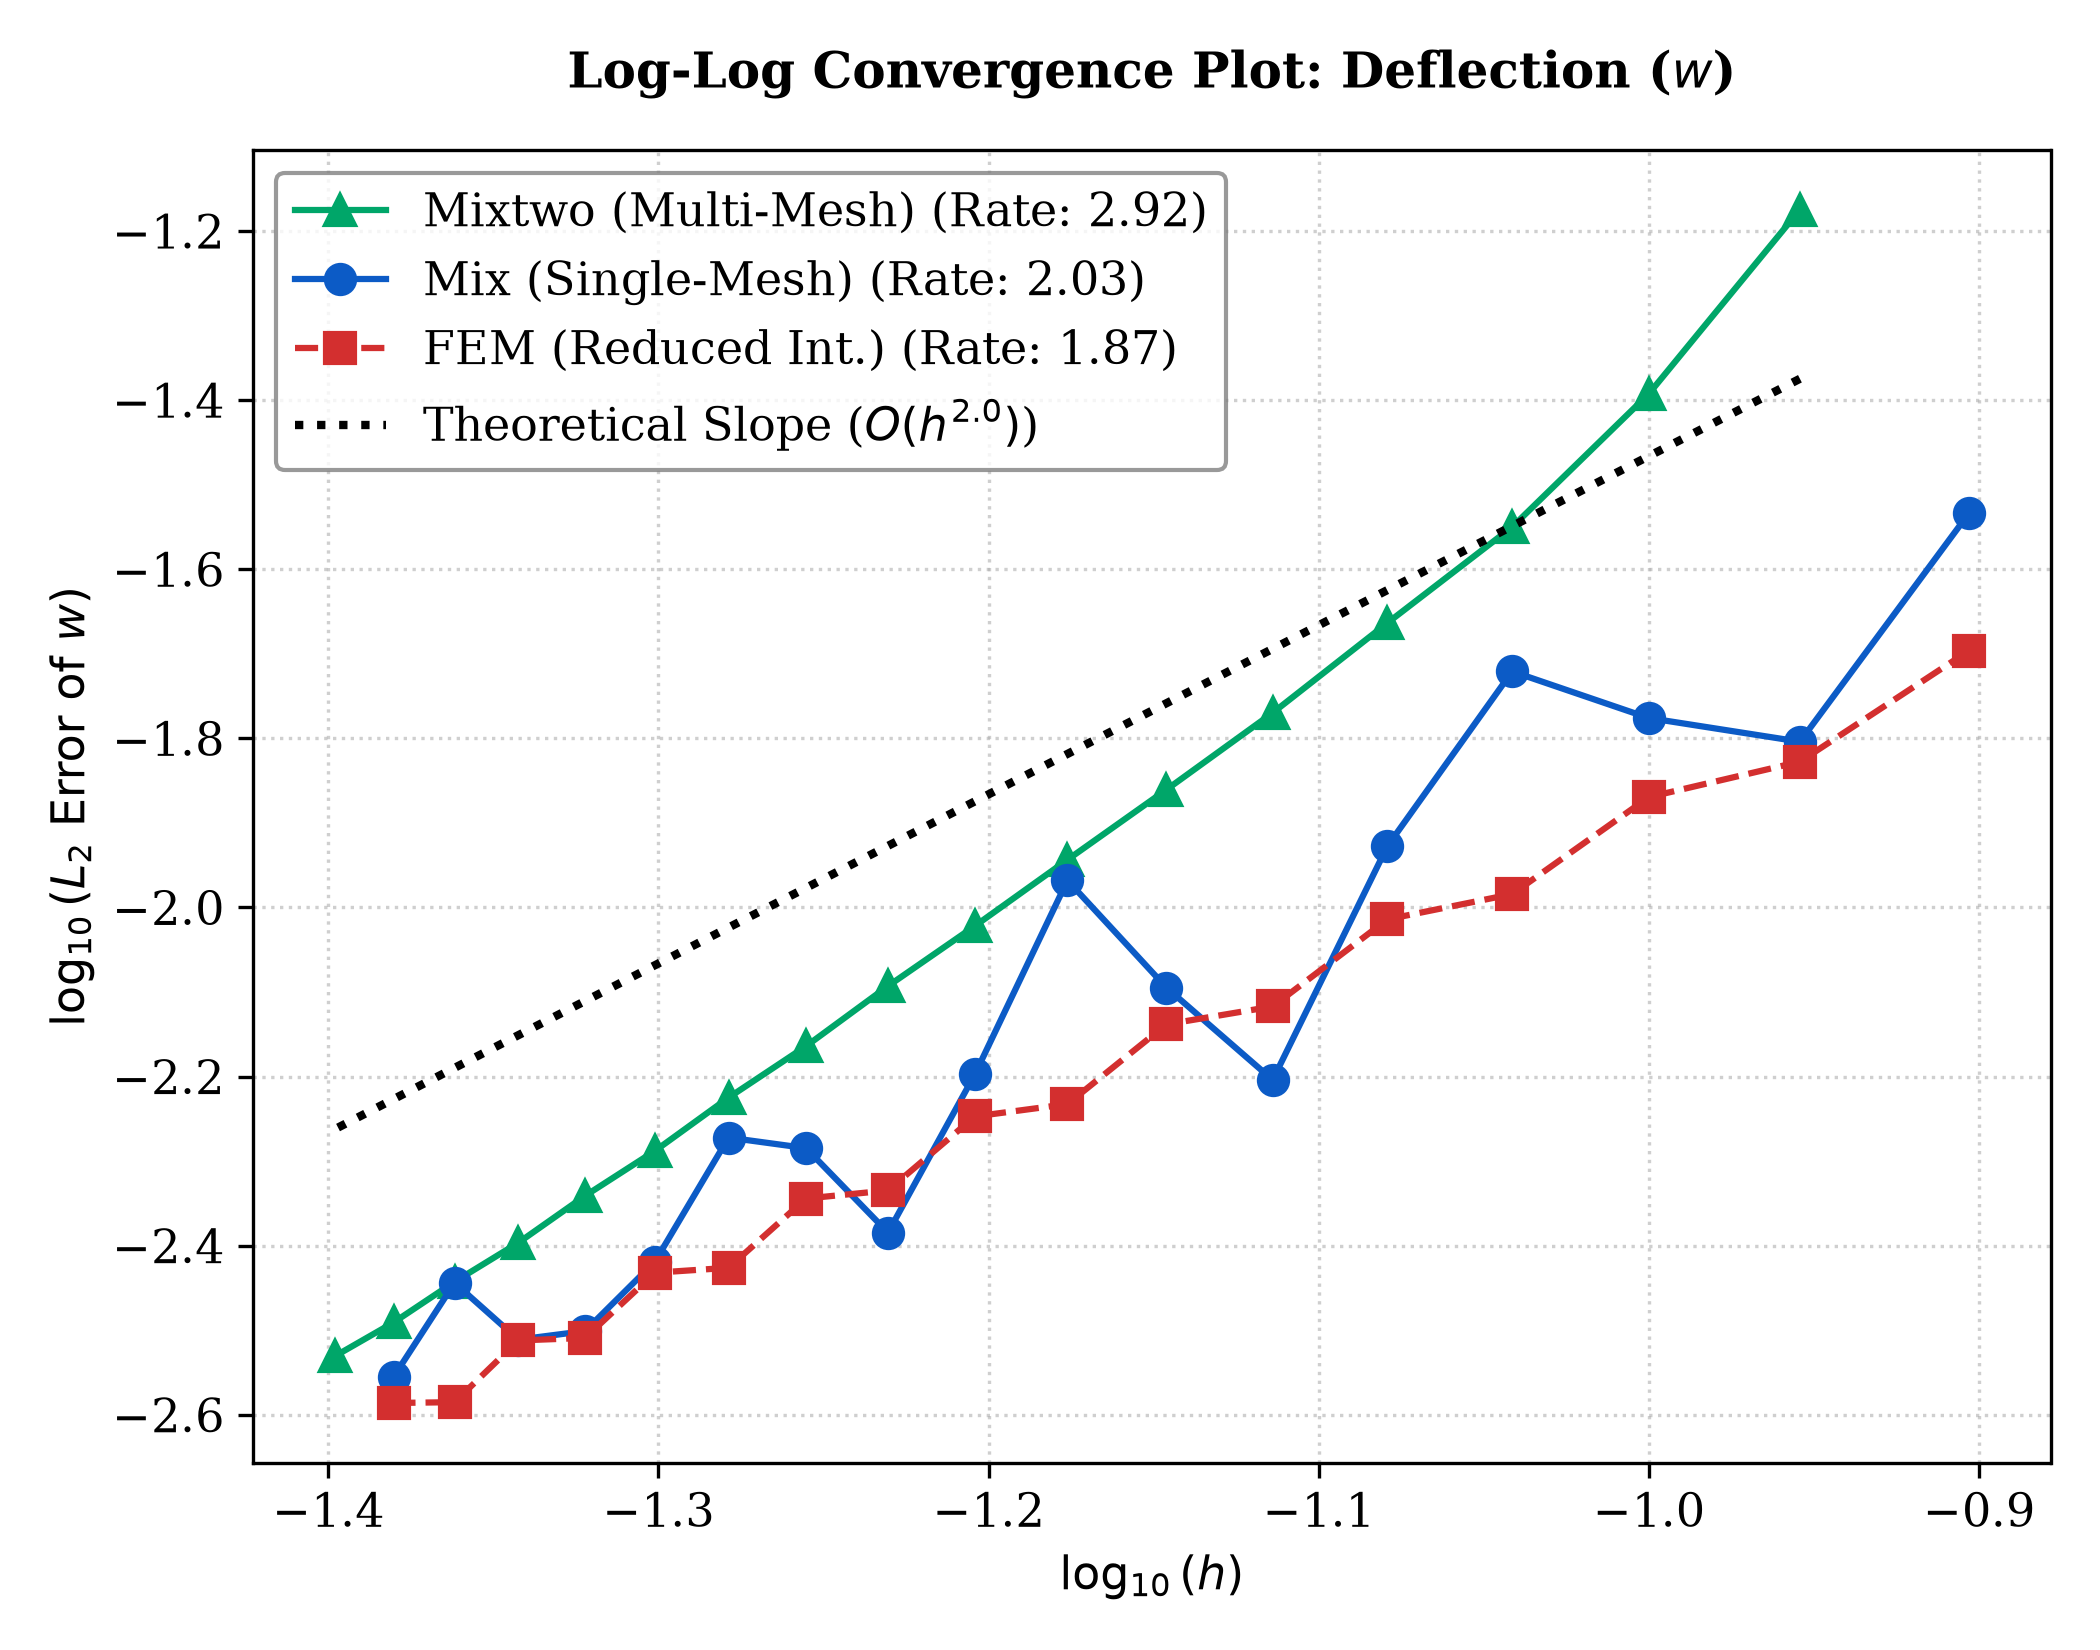
\includegraphics[width=0.45\textwidth]{plot_loglog_convergence_w.png}
    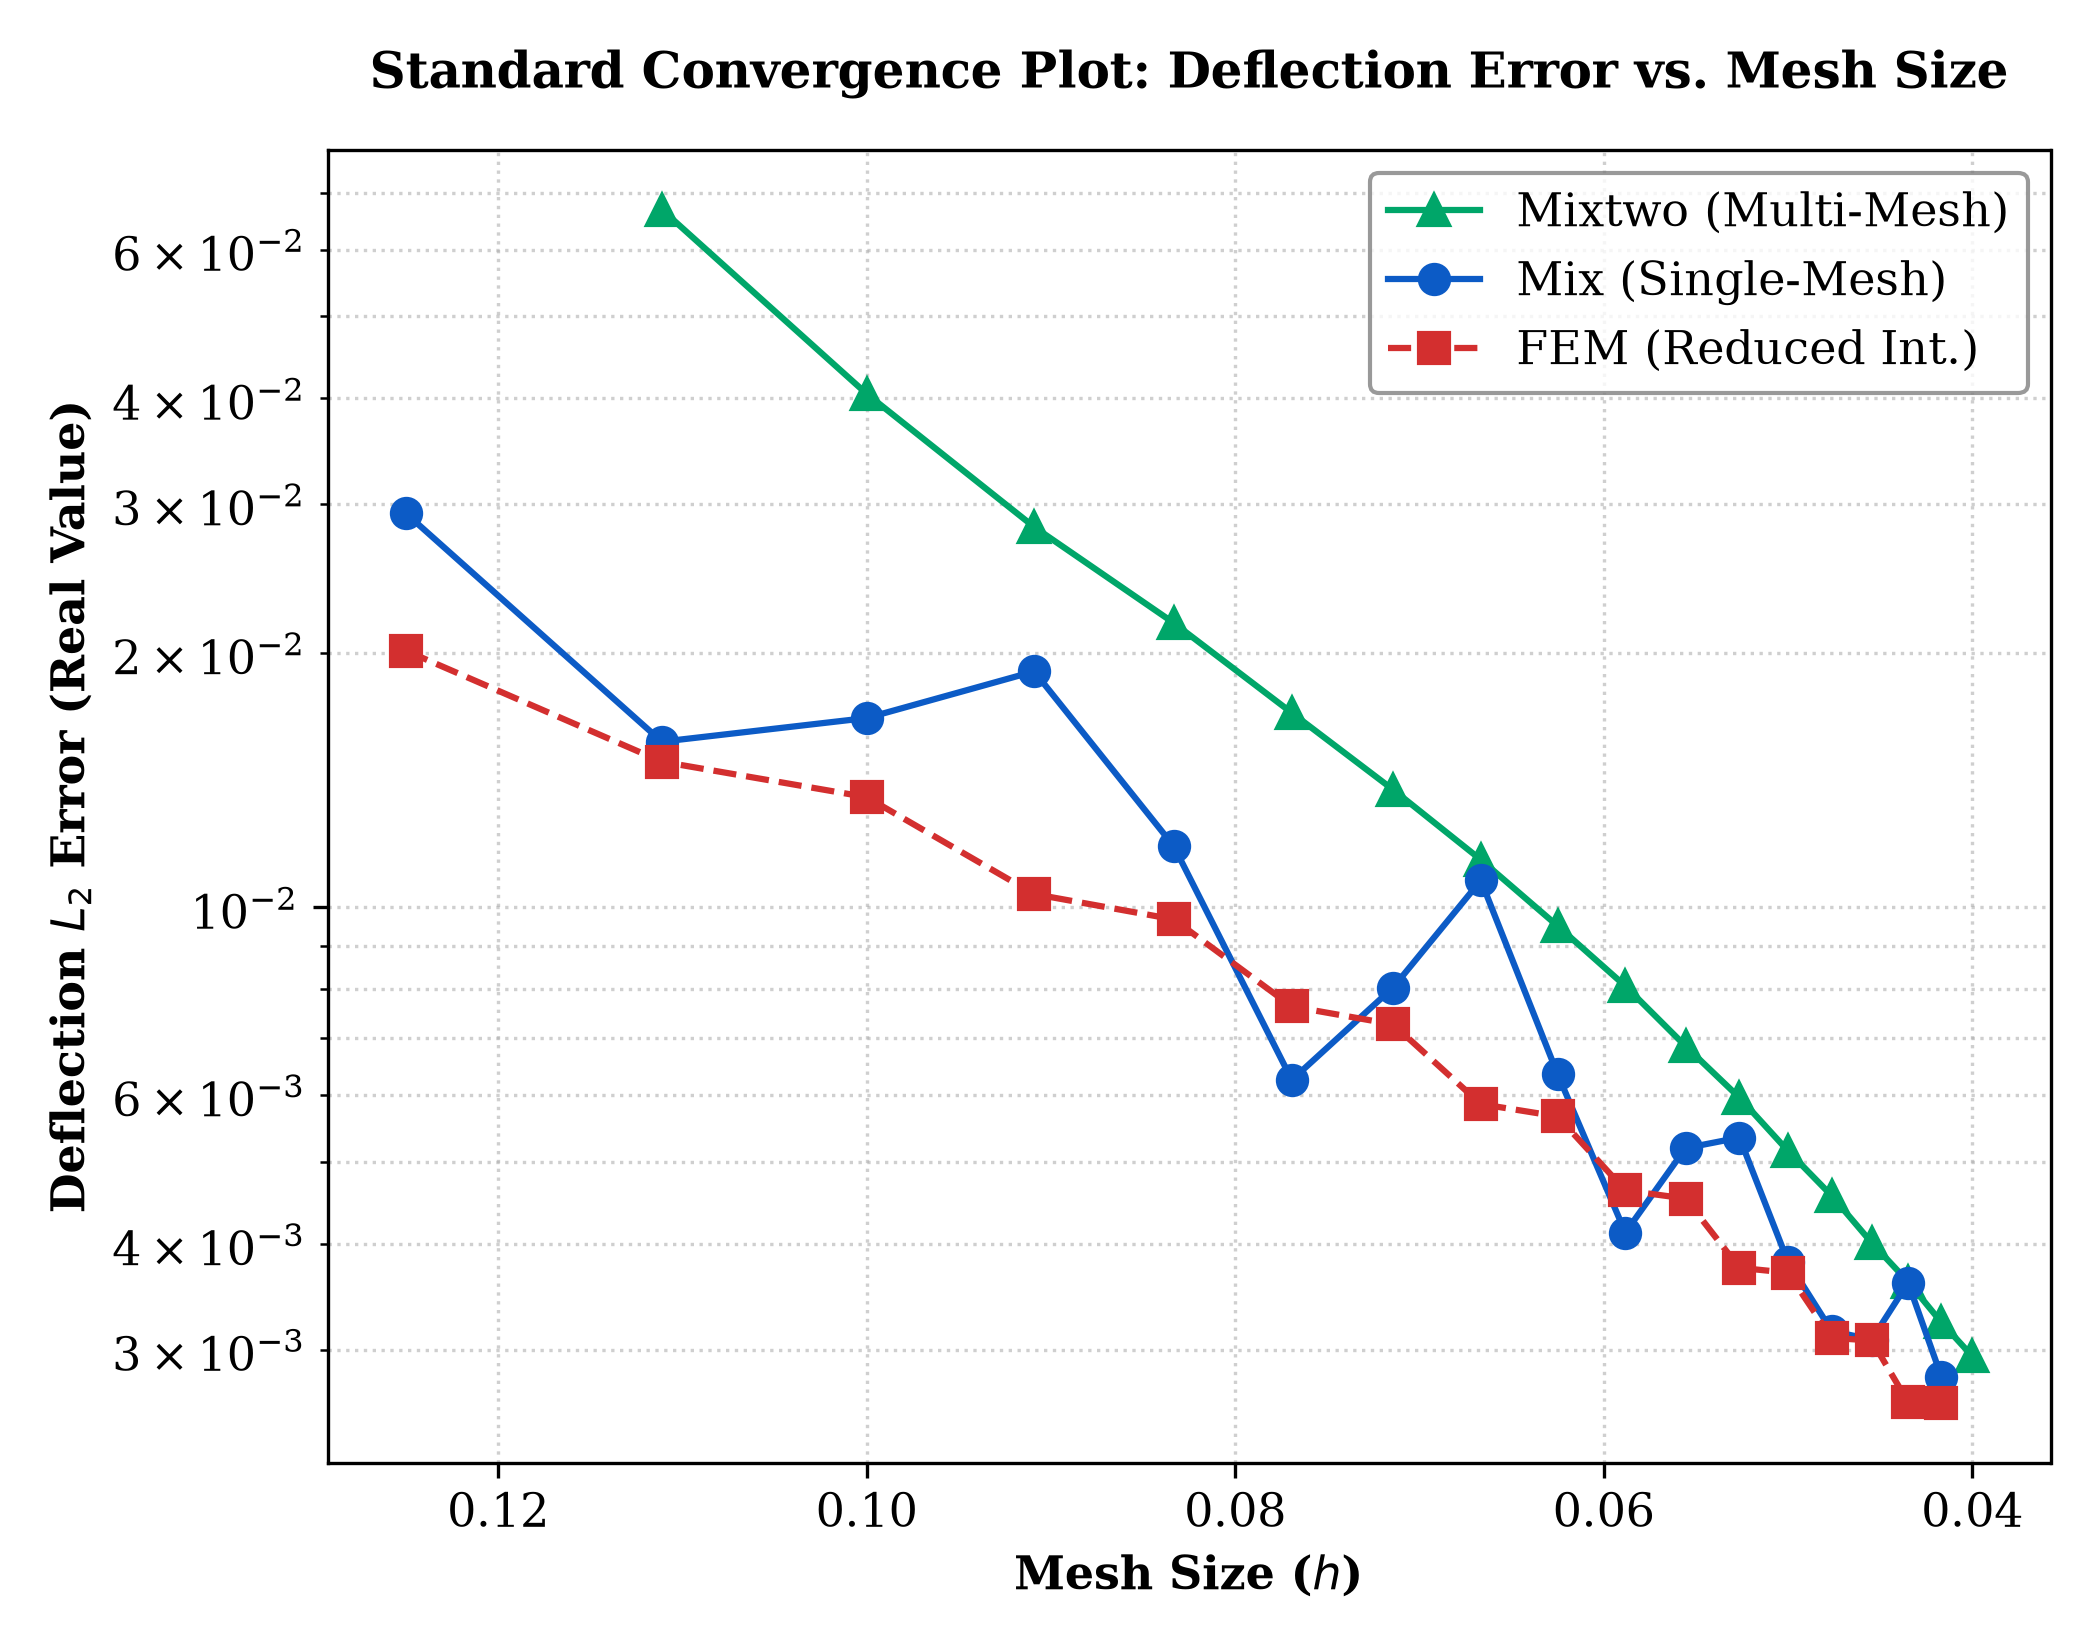
\includegraphics[width=0.45\textwidth]{plot_standard_convergence_w.png}
    \caption{位移場誤差收斂趨勢 (左：Log-Log Scale; 右：標準誤差圖)}
\end{figure}

\section{頻譜色散特性分析}
頻譜保真度指標（正規化頻率比值）定義為 $\text{Ratio} = \omega^h_{num} / \omega_{exact}$。數值 $1.0$ 代表與理論值完全吻合。

\begin{figure}[h]
    \centering
    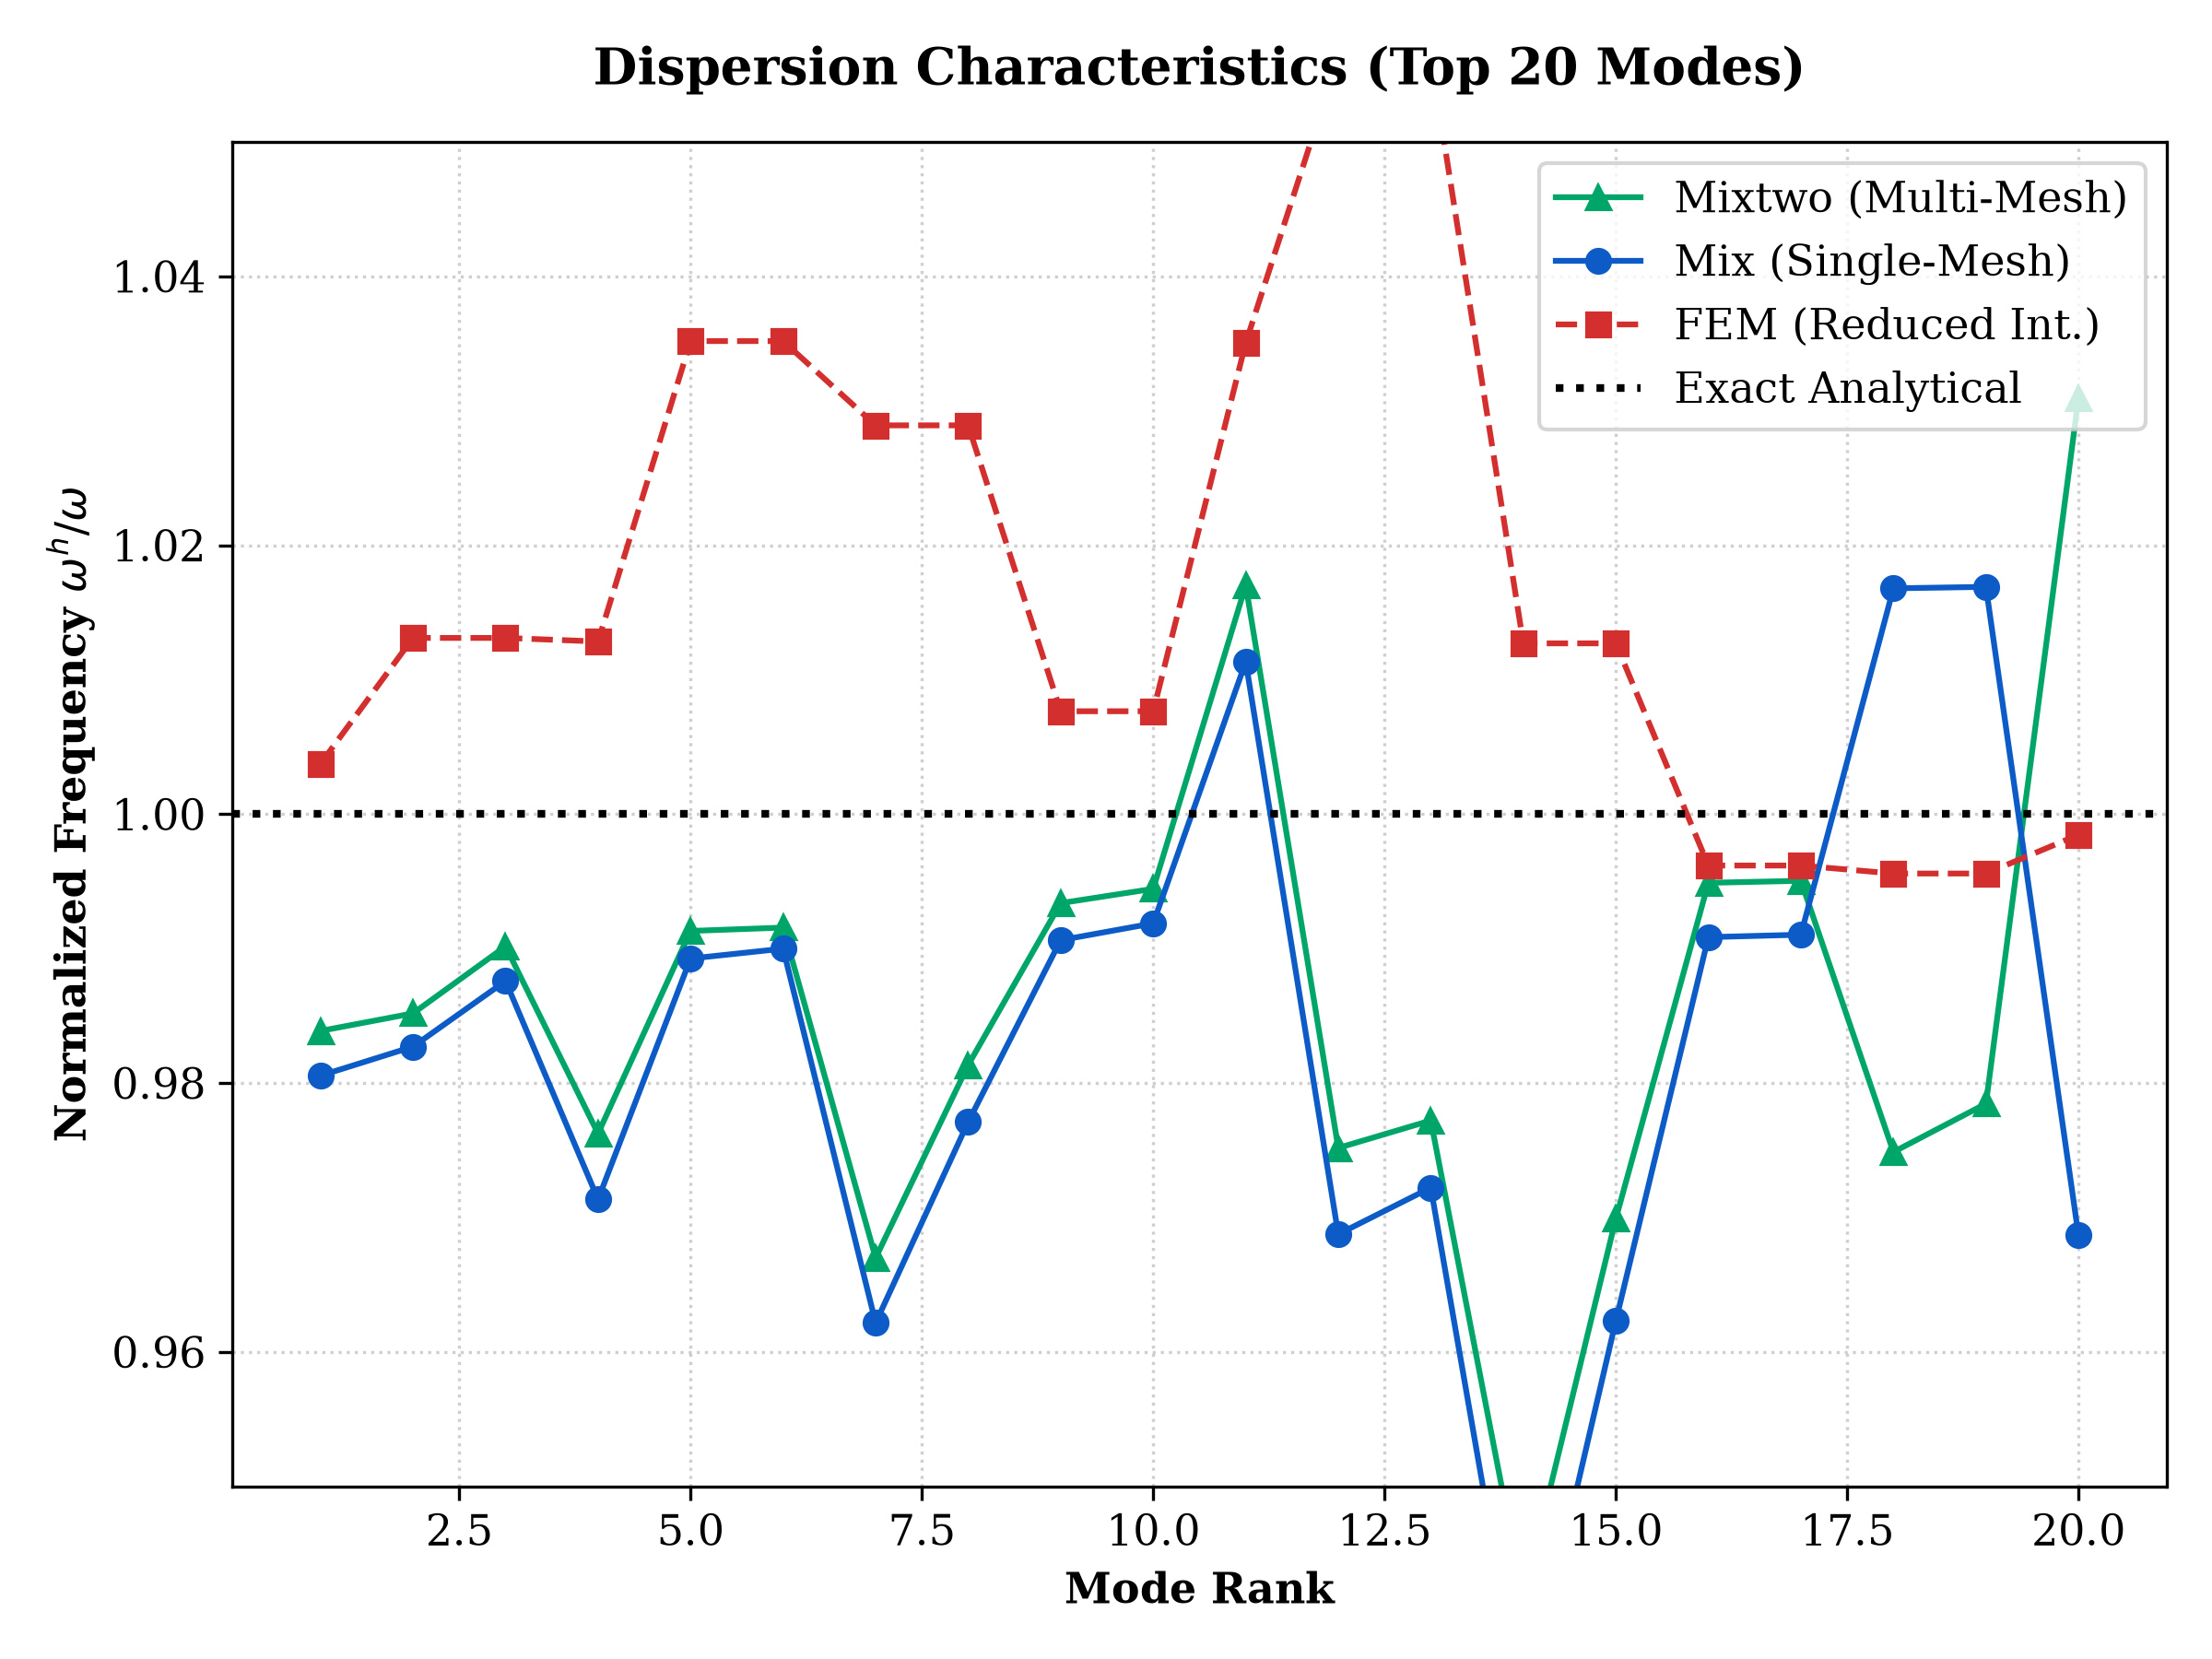
\includegraphics[width=0.6\textwidth]{plot_dispersion_top20.png}
    \caption{前 20 階模態之正規化頻率分佈}
\end{figure}

\subsection{數據解讀}
由圖可見，隨著模態階數增加，FEM 之頻率比值持續偏離 1.0，呈現「剛度過硬」趨勢。相比之下，Mixtwo 法在高階模態下仍能維持數值頻率接近理論值，證實其具備優異的抗色散能力 (Dispersion Robustness)，能有效捕捉高頻波之物理行為。

\section{結論}
本報告综合分析顯示，Mixtwo 方法透過網格解耦策略，成功突破了傳統 FEM 的收斂速率瓶頸，並在高頻區域展現了優異的頻譜保真度。基於數據對比，各方法之適用建議如下：
\begin{itemize}
    \item \textbf{FEM}：適用於計算資源受限、僅需初步結構動態特徵之簡單工程問題。
    \item \textbf{Mixtwo}：性能最優，適用於要求高頻頻譜精確度、結構幾何複雜或需嚴格誤差控制之場景。
\end{itemize}

\end{document}
